\documentclass[runningheads]{llncs}
\usepackage[utf8]{inputenc}
\usepackage{amsmath}
\usepackage{amsfonts}
\usepackage{subfiles}
\usepackage{amssymb}
\usepackage{csquotes}
\usepackage[numbers, sort, comma, square]{natbib}
\usepackage{changepage}
\usepackage{graphicx}
\usepackage{placeins}
\usepackage{xr}
\usepackage{tabularx}
\usepackage{lscape}
\usepackage{hyperref}
\usepackage{tablefootnote}
\usepackage{fancyhdr}
\usepackage{hyperref}
\newenvironment{jumpin}{\begin{adjustwidth}{0.3in}{}}{\end{adjustwidth}}


\begin{document}
\title{Document Embedding for Scientific Articles:\newline A validation of word embeddings}
\titlerunning{Document embedding for Scientific Articles}

\author{H.J. Meijer\inst{1,2}\orcidID{0000-1111-2222-3333} \and
R. Karimi\inst{2}\orcidID{1111-2222-3333-4444}}
\authorrunning{H.J. Meijer et al.}

\institute{University of Amsterdam, Science park 904, 1012WX Amsterdam, The Netherlands \and
Elsevier, Radarweg 29, 1043 NX Amsterdam, The Neterlands
\email{meijerarjan@live.nl, r.karimi@elsevier.com}}
\maketitle

\begin{abstract}
\subfile{Parts/Abstract/Abstract.tex}

\keywords{Word Embedding  \and Document Embedding \and Article Embedding \and Journal Embedding \and Embedding Visualization \and Embedding Validation.}
\end{abstract}
\section{Data}
For this research we used a dataset consisting of $186.962.354$ tokens. These tokens have been collected from $1.391.543$ articles which have been published in $3.759$ distinct journals. In our dataset, each article is represented with a title and an abstract.
\subsection{Sets}
\subsubsection{Embeddings}
For our research we used multiple embeddings (referred to as "sets"). These embedding sets are: the default embedding; as produced by the Word2Vec model and TF-IDF weighted embeddings (referred to in figures as \textit{embedding}). We used 4 variants of TF-IDF weighted embeddings: 
\begin{itemize}
\item{TF-IDF embedding (\textit{TFIDF\_embedding}); all words, weighted with the TF-IDF score, averaged to create an article embedding.}
\item{10K embedding (\textit{10K\_embedding}); TF-IDF weighting limited to the top 10.000 most occurring tokens.}
\item{5K embedding (\textit{5K\_embedding}); TF-IDF weighting limited to the top 5.000 most occurring tokens.}
\item{1K 6K embedding (\textit{1K\_6LK\_embedding}); TF-IDF weighting limited to the top 1.000 till 6.000 most occurring tokens.}
\end{itemize}
\subsubsection{TFIDF}
We furthermore used 3 TF-IDF sets, to create these sets we used the TF-IDF model and a hasher from the PySpark MlLib\footnote{\url{http://spark.apache.org/docs/2.0.0/api/python/pyspark.mllib.html}.}. We controlled these sets in two ways, (a) adjusting vocabulary size of the input and (b) adjusting the number of hashbuckets. We label the TF-IDF sets as follows: "vocabulary size / number of hash buckets", we furthermore indicate 1.000 as 1K. Thus, we label the TF-IDF configuration that has a vocabulary size of 10.000 and 10.000 hash buckets as TF-IDF 10K/10K. To select the TF-IDF sets, we measured and memory usage of multiple TF-IDF configurations. These results can be seen in Figures~\ref{figure:tfidfPerformance} and~\ref{figure:tfidfMemory}, in this figure we can see that the performance on both title and abstract stagnates; the same is true for the memory usage, although the memory usage does not stagnate as fast as the performance. Given these results, we selected the 10K/10K, 10K/5K and 5K/5K configurations for our research.
\begin{figure}[hbt]
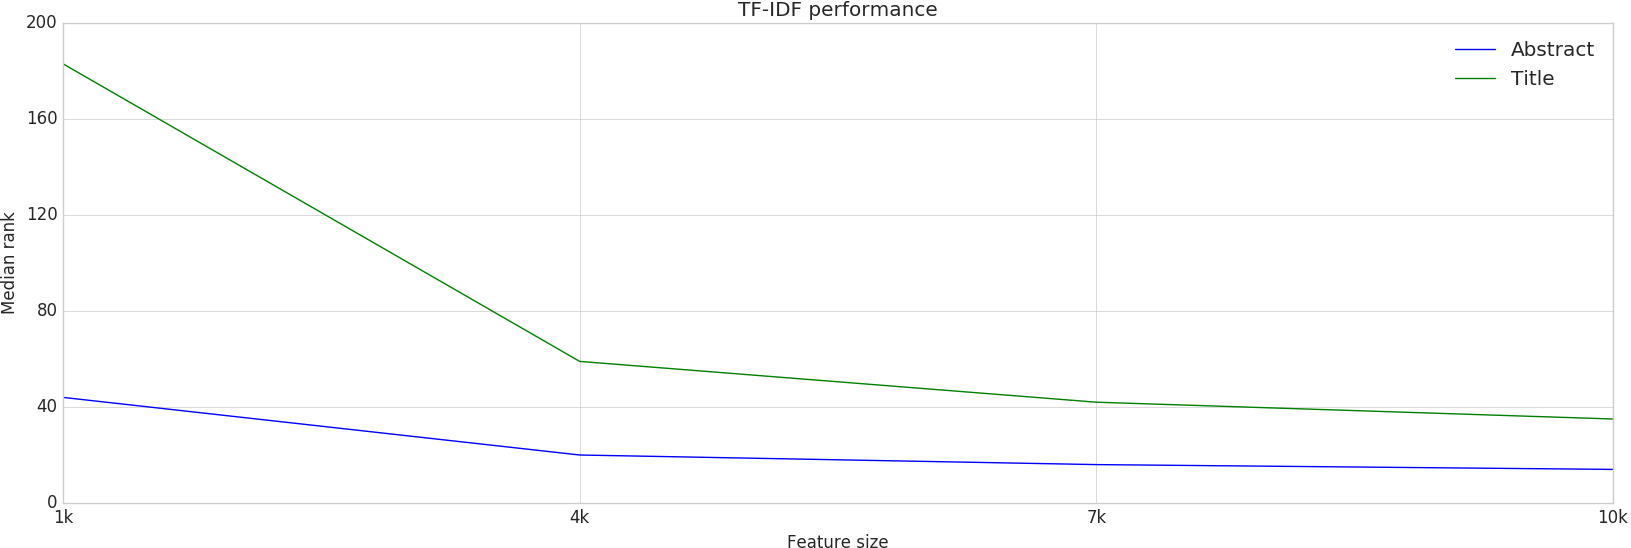
\includegraphics[width=5in]{Plots/tfidf_selection_plot_performance}
\caption{TF-IDF performance on title and abstract.}\label{figure:tfidfPerformance}
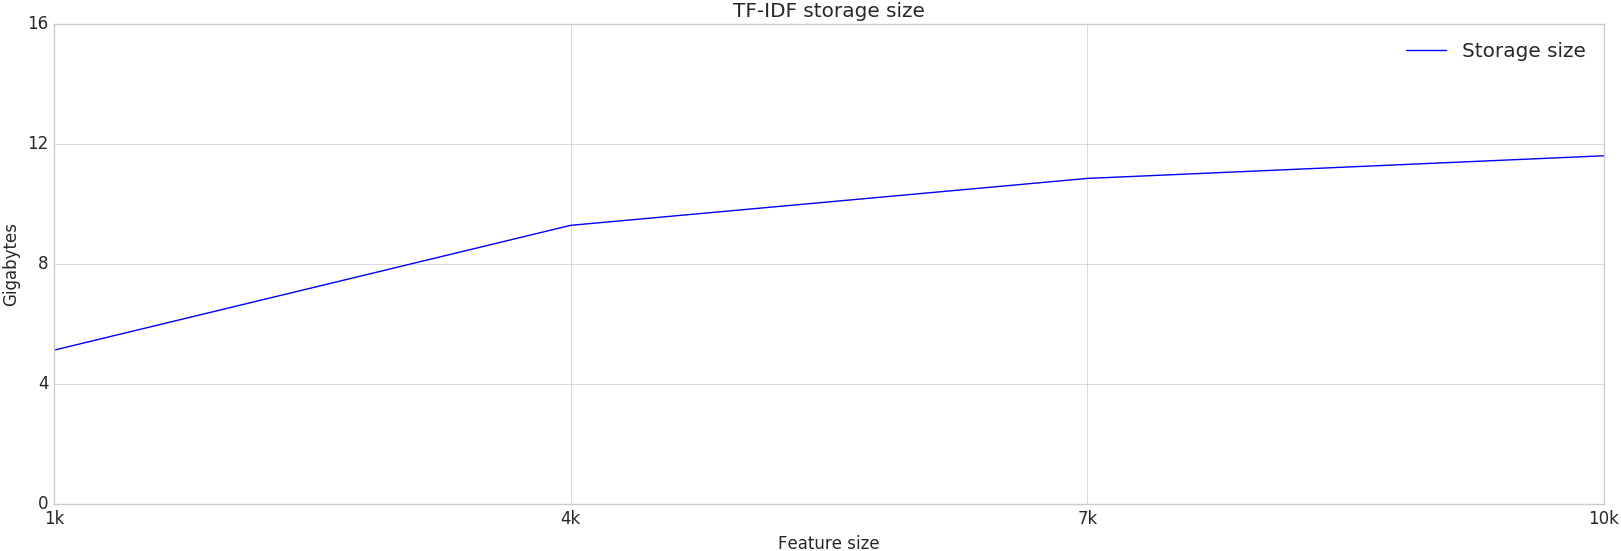
\includegraphics[width=5in]{Plots/tfidf_selection_plot_memory}
\caption{TF-IDF memory usage for title and abstract combined.}\footnote{We combined the memory usage of the titles and abstracts since the titles and abstract are created together and share their feature vector size.}\label{figure:tfidfMemory}
\end{figure}
\section{Methodology}

%\begin{theorem}
%This is a sample theorem. The run-in heading is set in bold, while
%the following text appears in italics. Definitions, lemmas,
%propositions, and corollaries are styled the same way.
%\end{theorem}
%
% the environments 'definition', 'lemma', 'proposition', 'corollary',
% 'remark', and 'example' are defined in the LLNCS documentclass as well.
%
%\begin{proof}
%Proofs, examples, and remarks have the initial word in italics,
%while the following text appears in normal font.
%\end{proof}
\citep{EBruniMENCollection}
\bibliographystyle{splncs04}
\bibliography{Bibliography}
\end{document}
